% displayname : Ondes mécaniques unidimensionnelles
\documentclass[12pt,fancy]{cours}
\Chapit{6}{1}
\begin{document}
\maketitre[***]{
  Nous commençons à étudier la physique des ondes sur les phénomènes propagatifs les plus simples : les phénomènes non dispersifs. Comme premier exemple, nous étudions les ondes mécaniques unidimensionnelles: ondes transverses le long d'une corde, puis ondes longitudinales dans les solides déformables. Tous les phénomènes non dispersifs obéissent à l'équation de d'Alembert, dont nous discuterons les propriétés et solutions.
}
{
\item Cours de Signaux 1 et 3 - 0
\item Documents de cours Signaux 1 - 1 et 2
\item TD Signaux 1 et 3
}

%%%%%%%%%%%%%%%%%%%%%%%%%%%%%%%%%%%%%%%%%%%%%%%%%%%%%%%%%%%%%%%%%%%%%%%%%%
\section{Ondes transverses : la corde vibrante}
\begin{definition}[Onde]\label{def:}
  Une \imp{onde} est la propagation au cours du temps d'une perturbation dans l'espace.
\end{definition}
 On distingue deux types d'ondes en fonction de la direction de la perturbation par rapport à la direction de propagation de l'onde.
\begin{enumerate}
  \item Une \imp{onde transverse} est une onde pour laquelle la perturbation est orthogonale à la direction de propagation de l'onde.
  
  \udl{Exemples} : une corde de guitare vibrante, une onde sismique de cisaillement, une onde électromagnétique polarisée rectilignement.
  \item Une \imp{onde longitudinale} est une onde pour laquelle la perturbation est parallèle à la direction de propagation de l'onde. 
  
  \udl{Exemples} : une onde sonore dans un fluide, une onde sismique de compression.
\end{enumerate}
Dans ce chapitre, nous discutons de deux ondes mécaniques unidimensionnelles : les ondes transverses le long d'une corde, et les ondes acoustiques, dans les solides, qui sont longitudinales.
\label{sec:corde}
\subsection{Modèle de la corde vibrante}
Soit une corde horizontale tendue (corde de guitare) initialement au repos. La corde est écartée d’une très petite distance transversalement par rapport à sa position d'équilibre (Fig.~\ref{fig:corde_vibrante}). On souhaite déterminer comment cette perturbation se propage dans l’espace et le temps.

L'étude est menée dans le référentiel du laboratoire supposé galiléen. Soit $\ex$ la direction horizontale (abscisse $x$), et $\ey$ la verticale ascendante (ordonnée $y$). L'onde de \important{transverse} car la perturbation (selon $\vv{e_y}$) est orthogonale à la direction de propagation de l'onde (selon $\vv{e_x}$). Voir \Fig{transverse} pour d’autres  ondes transverses. On ne prend pas le poids de la corde en compte, dont la direction est orthogonale au mouvement de la perturbation, ou négligeable devant la composante verticale de la tension de la corde.
% Autrement dit, $\vv{e_x}$ indique la direction de la corde au repos et $\vv{e_y}$ la direction transverse selon laquelle a lieu la perturbation mécanique .

\begin{figure}[H]
\centering

\includegraphics[width=\textwidth]{corde_vibrante.pdf}
\caption{Étude de la corde vibrante. Le schéma de droite représente un agrandissement d'une portion élémentaire de corde de longueur $\d x$.}
\label{fig:corde_vibrante}
\end{figure}

\noindent
Les hypothèses de l'étude sont les suivantes.
%:\footnote{Comme en mathématiques, les conditions d'applications d'un résultat sont au moins aussi importantes que le résultat lui-même. Il faut bien mémoriser les hypothèses.}
\begin{enumerate}[label=\fbox{H\arabic*}]
\item On néglige toute source de \important{dissipation}.
\item La corde est \imp{filiforme} : on la modélise par un fil homogène de masse linéique $\mu=m/L$.
\item La corde est \imp{infiniment souple} (sans raideur) : la force de tension est tangente à la corde.
\item L'ébranlement de la corde est \imp{faible} :  on se place dans l'approximation des \important{petits angles} $\alpha\ll 1$, où $\alpha$ désigne l'angle entre la tangente à la corde et l'horizontale. Autrememt dit, le déplacement $y(x,t)$ est purement transversal et petit devant la longueur $L$ de la corde, soit $y(x,t)\ll L$.
% En notant que $\tan\alpha=\frac{\partial y}{\partial x}$, dans l'hypothèse des petites déformations, on aura donc $\frac{\partial y}{\partial x}\ll 1$ et de plus $\abs{y(x,t)}\ll L$.
%\item le mouvement de la corde a lieu dans un plan à $z=\cte$, en particulier on \important{néglige tout mouvement de rotation} de la corde dans un plan normal à la direction horizontale.
\end{enumerate}

\begin{prop}[Modèle de la corde vibrante]\label{prop:mod_corde}
On étudie les faibles déplacements sans dissipation d’une corde filiforme homogène et sans raideur.
\end{prop}

On définit $\vv{T_{\rm{g}}}(x,t)$, la tension que la portion de corde à \emph{gauche} de l'abscisse $x$ exerce sur la portion située entre les abscisses $x$ et $x + \d x$. De même, on définit $\vv{T_{\rm{d}}}(x,t)$ la tension que la portion de corde à \emph{droite} de l'abscisse $x$ exerce sur la portion située entre les abscisses $x$ et $x + \d x$. D’après le principe des actions réciproques, $\vv{T_{\rm{d}}}(x,t) = - \vv{T_{\rm{g}}}(x,t)$.
%On note $T$ la norme

\subsection{Équation d'onde de d'Alembert}

\begin{methode}[Établir l’équation de la corde vibrante]
  \item	Appliquer le PFD à un élément de corde de longueur $\d x$.
  \item Projeter suivant $\ex$ et montrer que la tension $T$ est constante si $\alpha \ll 1$.
  \item Projeter suivant $\ey$ et relier l’accélération $\dr{y}{x}$ en fonction de la tension $T$ et de $\dr{\alpha}{x}$.
  \item Exprimer l’angle $\alpha$ en fonction de la déformation $y(x,t)$.
  \item Simplifier et obtenir l’équation de d’Alembert.
\end{methode}

\begin{enumerate}
  \item 
  Pour déterminer le déplacement de cette perturbation, on doit appliquer un théorème de la mécanique. Ici, nous appliquons le PFD à un élément de corde de longueur $\d x$ et de masse $\d m = \mu \d x$,
  \begin{equation}
    \d m \Vec{a} =  \mu\d x\frac{\partial^2 y}{\partial t^2}(x,t)\vv{e_y} = \vv{T_{\rm{d}}}(x+\d x,t)+\vv{T_{\rm{g}}}(x,t) = \vv{T_{\rm{d}}}(x+\d x,t) - \vv{T_{\rm{d}}}(x,t).
  \end{equation}
  % Or la force exercée au point d'abscisse $x$ par la partie située à gauche est égale à l'opposée celle exercée en ce même point par la partie située à droite (actions réciproques\footnote{On peut aussi appliquer le PFD en un point (système de masse nulle) pour établir ce résultat.}), autrement dit $\vv{T_{\rm{g}}}(x,t)=-\vv{T_{\rm{d}}}(x,t)$.
 \item Projetons sur $\ex$ :% le PFD donne donc
 \begin{equation}
 0=T_{\rm{d}}(x+\d x,t)\cos\alpha(x+\d x,t)-T_{\rm{d}}(x,t)\cos\alpha(x,t).
 \end{equation}
 Comme les angles sont petits, $\cos\alpha(x+\d x,t)\simeq \cos\alpha(x,t) =  1 + O(\alpha^2)$, et donc la tension de la corde $T_{\rm{d}}(x,t)\simeq T= \cte$ est environ constante.
 % au premier ordre. On note alors plus simplement
  \item Projetons sur $\vv{e_y}$ :%donne d'autre part
 \begin{align}
 \mu\d x\frac{\partial^2 y}{\partial t^2} = T\left[\sin\alpha(x+\d x,t)-\sin\alpha(x,t)\right] & = T\left[\alpha(x+\d x,t)-\alpha(x,t)\right] + O(\alpha^2) \\ & \simeq  T\frac{\partial \alpha}{\partial x}(x,t)\d x +  O(\d x^2).
\end{align}
\item 
Or par définition de $\alpha$, on a la propriété géométrique
\begin{equation}
 \alpha \simeq \tan\alpha = \frac{\partial y}{\partial x}.
\end{equation}
\item 
Après simplification par $\d x$,
\begin{equation}
  \mu\frac{\partial^2 y}{\partial t^2}(x,t)=T\frac{\partial^2 y}{\partial x^2}(x,t).
\end{equation}
Cette équation se met sous la forme d'une équation de d'Alembert
\begin{equation}
  \frac{\partial^2 y}{\partial x^2}-\frac{1}{c^2}\frac{\partial^2 y}{\partial t^2}=0\qquad\text{avec}\quad \boxed{c=\sqrt{\frac{T}{\mu}}},
\end{equation}
où $c$ désigne avec la célérité des ondes mécaniques transverses le long de la corde, et où la dépendance en $(x,t)$ est sous-entendue pour $y$.
\end{enumerate}


\begin{figure}[H]
  \centering
     \subfigure[]{
     
\includegraphics[height=0.2\textwidth]{houle.jpeg}
     }
     \subfigure[]{
     
\includegraphics[height=0.2\textwidth]{Swave.png}
     }
     \subfigure[]{
     
\includegraphics[height=0.2\textwidth]{electromag_wave.pdf}
     }
     \caption{Autres exemples d’ondes transverses de nature (a,b) mécanique et (c) électromagnétique. (a) Houle. (b) Onde sismique de cisaillement S. (c) Onde électromagnétique (ici polarisée rectlignement).}
     \label{fig:transverse}
   \end{figure}


 \begin{theorem}[Équation de D’Alembert]
	 L’équation de propagation d’une perturbation $y(x,t)$ le long d’une corde vibrante vérifie
 	$$
 \frac{\partial^2 y}{\partial x^2}-\frac{1}{c^2}\frac{\partial^2 y}{\partial t^2}=0,
	$$
	où $c>0$ désigne la célérité de l’onde (en $\SI{}{m.s^{-1}}$).
 \end{theorem}

 \begin{theorem}[Célérité des ondes de la corde vibrante]\label{form:}
  La célérité d'une déformation transverse d'une corde vaut
  \begin{equation*}
  c=\sqrt{\frac{T}{\mu}},
  \end{equation*}
  avec $T$ la tension de la corde, et $\mu$ sa masse linéique.
 \end{theorem}


  


 % \begin{remarque}
 % La célérité dans le milieu s'interprète qualitativement comme
 % \begin{equation}
 % c=\frac{\mathrm{raideur}}{\mathrm{inertie}}=\sqrt{\frac{T}{\mu}}.
 % \end{equation}
 % \end{remarque}

\section{Ondes longitudinales : onde acoustique dans un solide}

Nous étudions maintenant une autre onde mécanique régie par l'équation de d'Alembert : la propagation du son (onde acoustique ou sonore) dans les solides. Cette onde est \imp{longitudinale}, contrairement au déplacement d’une perturbation le long d’une corde.  D’un point de vue microscopique, l’onde met en vibration les atomes de proche en proche. Nous commençons donc par présenter un modèle discret d’un solide.
% : elle nécessite un support matériel pour se propager, en mettant en vibration les atomes de proche en proche, et ne peut donc pas se propager dans le vide. Dans la suite nous étudions un modèle simple pour décrire la propagation d'ondes acoustiques (sonores ou ultrasonores, donc audibles ou non) au niveau microscopique dans un solide supposé unidimensionnel (une tige métallique par exemple). L'étude des ondes acoustiques dans les fluides (liquides ou gaz) fera l'objet du chapitre suivant.

\subsection{Modèle discret: la chaîne de ressorts}
%\begin{figure}[h!]
%\centering
%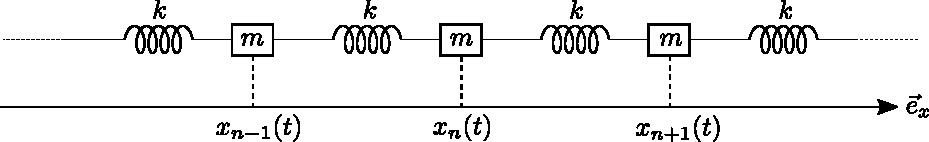
\includegraphics[width=0.85\textwidth]{Figures/chaine_ressorts.pdf}
%\caption{Modèle discret d'un solide vu comme une chaîne unidimensionnelle de masses et de ressorts identiques.}
%\end{figure}

\parag{Description du modèle}
On modélise un solide unidimensionnel par une chaîne de systèmes masse-ressort. On note respectivement $d$ et $x_n^{0}=nd$ la longueur des ressorts et la position de la $n^{\rm{ème}}$ masse, au repos.
Une onde acoustique est une perturbation mécanique qui modifie légèrement les positions des masses par rapport à l'équilibre en comprimant ou allongeant les ressorts. Soit $\xi_n(t)$ le déplacement (algébrique) induit par le passage de l'onde. La position de la masse $n$ s'écrit (\Fig{chaine_ressorts})
\begin{equation}\label{eq:xn}
  x_{n}(t)=x_n^{0}+\xi_{n}(t)=nd+\xi_{n}(t).
 \end{equation}
 % De la même manière, $x_{n\pm 1}(t)=(n\pm 1)d+\xi_{n\pm 1}(t)$. La situation au repos et lors du passage de l'onde lorsque les déplacements sont tous positifs est représentée en Fig.~\ref{fig:chaine_ressorts}.

\begin{figure}[H]
\centering

\includegraphics[width=0.85\textwidth]{chaine_ressorts_perturb.pdf}
\caption{Chaîne à l'équilibre (en haut) puis hors équilibre lors du passage de l'onde (en bas).}
\label{fig:chaine_ressorts}
\end{figure}

\parag{Équation de la dynamique} Pour établir l'équation d'onde vérifiée par le déplacement $\xi_n(t)$ de la masse $n$, la stratégie est la même que précédemment : appliquons le PFD à la masse $n$ dans le référentiel du laboratoire.

\begin{liste}
  \item Bilan des forces : tension $\Vec{T}_{g,n} = k (\ell_n - d) (-\ex) $ exercée par le ressort gauche sur la masse $n$ (car $-\ex$ pointe vers la gauche); tension $\Vec{T}_{d,n} =  k (\ell_{n+1} - d) (+\ex) $ exercée par le ressort droit sur la masse $n$ (car $+\ex$ pointe vers la droite). Les longueurs valent $\ell_n = x_{n}(t)-x_{n-1}(t)$ et  $\ell_{n+1} = x_{n+1}(t)-x_{n}(t)$, et donc d’après l’\Eq{xn}, on a
  $\Vec{T}_{g,n} = -k (\xi_{n}(t)-\xi_{n-1}(t)) \ex $ et $\Vec{T}_{d,n} =  k (\xi_{n+1}(t)-\xi_{n}(t)) \ex $.
  \item le PFD donne
  \begin{equation}
  \begin{split}
  m\frac{\d^2 x_{n}}{\d t^2}\vv{e_x} = m\frac{\d^2 \xi_{n}}{\d t^2}\vv{e_x}   = \Vec{T}_{g,n} + \Vec{T}_{d,n}   =-k(\xi_{n}(t)-\xi_{n-1}(t))\vv{e_x} +k(\xi_{n+1}(t)-\xi_{n}(t))\vv{e_x}
  \end{split}
  \end{equation}
  En simplifiant il vient
  % \begin{equation}
    \eqbox[]{
      \label{eq:eq_onde_discrete}
      m\frac{\d^2 \xi_{n}}{\d t^2}=k\left[\xi_{n+1}(t)+\xi_{n-1}(t)-2\xi_n(t)\right].
      }
      % \end{equation}
\end{liste}
L’\Eq{eq_onde_discrete} n’est pas encore une équation d’onde. En effet, ce n’est pas une équation fermée (elle fait interenir trois fonctions du temps différentes $\xi_{n-1}(t)$, $\xi_{n}(t)$ et $\xi_{n+1}(t)$). Ce problème se résout facilement en écrivant les équations associées à toutes les autres masses. S’il y a $N$ atomes, on aboutit à $N$ équations différentielles linéaires pour $N$ inconnues, ce qui forme un système résoluble. Mais surtout, une équation d’onde porte sur une fonction du temps $t$ et de \emph{l’espace} $x$. Comment passer des $\xi_n(t)$ à une fonction de $(x,t)$ ?
%
% Selon la direction horizontale orthogonale au poids, la masse $n$ subit deux forces des tensions des ressorts: une du ressort en commun avec la masse $n-1$ et une du ressort en commun avec la masse $n+1$. On suppose ici que les masses suivantes ne sont pas affectées, ce qui est légitime puisque nous avons supposé que l'onde modifie seulement légèrement la position autour de l'équilibre, donc $\xi_n(t)\ll nd$.
%
% Pour ne jamais se tromper sur le signe des tensions des ressorts, on écrit \JRouge{toujours} chaque force sous la forme
% \begin{equation}
% \vv{T}=-k\times \Delta l \times \vv{e}_{\rm{fixe}\rightarrow \rm{mobile}},
% \end{equation}
% où on détermine simplement l'allongement \important{algébrique} $\Delta l$ comme la longueur à l'instant $t$ moins la longueur à l'équilibre. Le vecteur directeur est dirigé de la partie supposée fixe sur la partie mobile, c'est-à-dire la masse étudiée. Cette formule est toujours valable, que les ressorts soient comprimés ou étirés. Ceci étant, il est conseillé de déplacer les masses toutes dans le même sens pour minimiser le nombre de signes moins (comme sur le schéma de la Fig.~\ref{fig:chaine_ressorts}).

% Appliquons la relation précédente: on suppose les masses $n+1$ et $n-1$ fixes, et on fait bouger la masse $n$, il vient alors
%
% (si vous réfléchissez en terme d'allongement et à partir du schéma, il est possible d'écrire directement la deuxième ligne).


\subsection{Approximation du continu}
Pour simplifier l'expression précédente, il faut revenir à la physique du problème. On cherche à décrire une onde sonore de longueur d'onde $\lambda$. On s’attend donc à ce que $\xi(x,t)$ ne varie sensiblement que sur des distances de l’ordre de $\lambda$ ou plus. Or $\lambda \gg d$ en pratique. Cela nous permet de définir une fonction $\xi(x,t)$ \guill{lisse} (en pratique $\mc{C}^2$ suffit) telle que $\xi(x_n(t),t) = \xi_n(t)$ pour tout $n$.
% Nous allons donc définir par passage à la limite continue une seule fonction $\xi(x,t)$, qui décrira le déplacement temporel de l'atome qui au repos est placé en $x=x_{n}^0=nd$. Nous définissons en fait ici un champ, en tout point de l'espace $x$ et du temps $t$, qui décrit l'évolution de la déformation lors du passage de l'onde.
% Nous faisons donc les changements suivants
% \begin{equation}
%      \begin{cases}
%      \xi_n(t)\rightsquigarrow \xi(x,t)\\
%      \xi_{n\pm 1}(t)\rightsquigarrow \xi(x\pm d,t).
%      \end{cases}
%      \end{equation}
En $x=x_n$, on a $\xi_n(t) = \xi(x,t)$, $\xi_{n+1}(t)=\xi(x+d,t)$ et $\xi_{n-1}(t)=\xi(x-d,t)$. L'Éq.~\eqref{eq:eq_onde_discrete} se réécrit alors
\begin{equation}
\label{eq:eq_onde_continue_sans_DL}
m\frac{\partial^2 \xi}{\partial t^2}(x,t)=k\left[\xi(x+d,t)+\xi(x-d,t)-2\xi(x,t)\right].
\end{equation}


  \begin{prop}[Approximation du continu]\label{prop:}
    Si la longueur d’onde $\lambda \gg d$ est grande devant la distance atomique $d$, 
    on peut définir une fonction déplacement $\xi(x,t)$ de catégorie $\mc{C}^2$ en $x$ telle que 
    $
    \xi(x_n(t),t) = \xi_n(t).
    $
    
  \end{prop}
  \begin{exemple}{Validité de l’approximation du continu}
    Les ondes sonores se propage dans les solides à une célérité typique $c \sim \SI{5}{km.s^{-1}}$. Que vaut la longueur d’onde pour une onde de fréquence $f = \SI{20}{kHz}$ (à la limite de l'audible) ? L’approximation du continu est-elle justifiée ?
    \examplesol{
       Pour une onde de fréquence $f = \SI{20}{kHz}$ (à la limite de l'audible), la longueur d'onde vaut $\lambda = c/f  \sim \SI{25}{cm}$. La distance inter-atomique est de l'ordre de $ d \sim \SI{e-10}{m}$, qui est minuscule par rapport à $\lambda$. On a donc 
       \eqbox{
  \lambda \gg d, } et l'approximation du continu est parfaitement justifiée.
    }
  \end{exemple}

  
  L’approximation du continu justifie aussi un développement de Taylor en $x$. À l’ordre 2 :
  \begin{equation}
  \xi(x\pm d,t) \simeq \xi(x,t)\pm d\frac{\partial \xi}{\partial x}(x,t)+\frac{d^2}{2}\frac{\partial^2\xi}{\partial x^2}(x,t).
  \end{equation}
  En substituant dans l'expression \eqref{eq:eq_onde_continue_sans_DL} il vient
   \begin{equation}
m\frac{\partial^2 \xi(x,t)}{\partial t^2}=kd^2\frac{\partial^2\xi(x,t)}{\partial x^2}.
  \end{equation}
  L'équation d'onde se met à nouveau sous la forme d'une équation de d'Alembert
  % \footnote{Ce n'est pas une coïncidence, car l'équation de d'Alembert décrit tous les phénomènes propagatifs non dissipatifs et non dispersifs à une dimension.} 
  
  % \begin{equation}
    \eqbox[]{
      \label{eq:onde_sonore}
      \frac{\partial^2\xi }{\partial x^2}-\frac{1}{c^2}\frac{\partial^2\xi}{\partial t^2}=0\qquad\mathrm{avec}\quad c=d\sqrt{\frac{k}{m}}.
    }
  % \end{equation}
 % \begin{remarque}
 % Comme dans le cas précédent, la célérité de l'onde acoustique dans le solide est représentée qualitativement par le rapport
 % \begin{equation}
 % c=\frac{\mathrm{raideur}}{\mathrm{inertie}}=d\sqrt{\frac{k}{m}}=\sqrt{\frac{k/d}{m/d^3}}.
 % \end{equation}
 % \end{remarque}

\subsection{Loi de Hooke}
L'expression de l’\Eq{onde_sonore} pour la célérité de l'onde n’est pas très utile, puisque les constantes $d, m$ et surtout $k$  du modèle microscopique ne sont pas directement mesurables. De plus, la raideur $k$ dépend du modèle choisi. Comment relier le modèle microscopique aux propriétés macroscopiques du matériau ? La loi de Hook permet de faire ce lien.


\parag{Loi de Hooke}
Supposons que l'on exerce une force de traction $\vv{F}=F \ex $ répartie uniformément sur la section $S$ d'un solide (Fig.~\ref{fig:Hooke}). Cette traction induit en général un allongement $\Delta \ell$ du solide dans la direction de traction $\ex$ par rapport à la longueur au repos $\ell_0$.
Tant que cette force n'est pas trop importante (régime de déformation linéaire), la force surfacique est proportionnelle à l'allongement relatif dans la direction de la force.

\begin{figure}[H]
\centering
\subfigure[]{\label{fig:}

\includegraphics[width=0.45\textwidth]{hooke.pdf}
}\hspace{1cm}
\subfigure[]{\label{fig:}

\includegraphics[scale=1.1]{young.pdf}
}
\caption{Étirement d'un solide et loi de Hooke. (a) Définition de la contrainte (force surfacique $F/S$) et de la déformation (allongement relatif $\Delta \ell/\ell_0$). (b) Relation empirique entre contrainte et déformation.}
\label{fig:Hooke}
\end{figure}

\begin{theorem}[Loi de Hooke]\label{form:}
  Dans le régime élastique, la relation entre contrainte et déformation est linéaire,
  \begin{equation*}
  \frac{F}{S}=E\,\frac{\Delta \ell}{\ell_0},
\end{equation*}
où la constante $E$ (en \SI{}{GPa}) est appelée \important{module de Young}.
\end{theorem}

% Il s'agit de la loi de Hooke. La constante $E$, homogène à une pression et généralement exprimée en \SI{}{GPa}, est appelée le \important{module de Young} du matériau.

% On peut trouver sa valeur pour un matériau donné dans des tables.
% Plus ce module de Young est petit, plus le matériau est facilement étirable. Pour le caoutchouc, typiquement les valeurs varient de 0,001 à 0,1 \SI{}{GPa}, pour le bois \SI{10}{GPa} et pour l'acier \SI{200}{GPa}.
\begin{table}[H]
  \centering
  \begin{tabular}{|c|c|c|c|c|}
    \hline
    Matériau & Caoutchouc & Bois & Acier & Diamant \\
    \hline
    E (GPa) & \num{0.001} - \num{0.1} & 10 & 200 & 1000 \\
    \hline
  \end{tabular}
\end{table}
  

\parag{Lien avec le modèle microscopique}
% La relation précédente va nous permettre d'exprimer la vitesse de l'onde mécanique en fonction des paramètres macroscopiques mesurables.
Nous avons considéré une chaîne unidimensionnelle d'atomes, distants de $d$. Considérons une section carré d’une chaîne d’atomes, de surface $S=d^2$. La force de traction microscopique qui s’exerce sur cette section vaut $F=k(\xi_{n+1}-\xi_n)\simeq kd\frac{\partial\xi}{\partial x}$. La contrainte vaut donc
\begin{equation}
  \frac{F}{S} = \frac{k}{d} \dr{\xi}{x}.
\end{equation}
 % est répartie sur une surface élémentaire $S$ qui contient $\frac{S}{d^2}$ maillons. La force surfacique résultante s'écrit donc $\frac{k}{d}\frac{\partial\xi}{\partial x}$.
 Il s'agit de la loi de Hooke avec $E=\frac{k}{d}$. De plus, la masse volumique du matériau s'écrit $\rho=\frac{m}{d^3}$ et donc la célérité de l'onde s'écrit comme $c=\sqrt{\frac{k d^2}{m}} =\sqrt{\frac{E}{\rho}} $.
 \begin{theorem}[Célérité du son dans un solide]\label{form:}
   La célérité des ondes acoustiques dans un solide vaut
   \begin{equation*}
   c=\sqrt{\frac{E}{\rho}},
   \end{equation*}
   avec $E$ le module de Young, et $\rho$ la masse volumique.
 \end{theorem}

\section{Solutions de l'équation de d’Alembert}
Dans la suite on considère une équation de d'Alembert unidimensionnelle sur la grandeur $s(x,t)$ :
\begin{equation}
   \frac{\partial^2 s}{\partial x^2}-\frac{1}{c^2}\frac{\partial^2 s}{\partial t^2}=0.
\end{equation}
% Les solutions sont par définition des \imp{ondes planes}, car $s(x,t)$ ne dépend que d'une coordonnée spatiale $x$.
\begin{definition}[Onde plane]\label{def:}
  Un \imp{onde plane} est une perturbation $y(x,t)$ qui dépend d'une seule variable cartésienne $x$.
\end{definition}
\subsection{Ondes planes progressives (OPP)}

\begin{definition}[OPP]
 Une \imp{onde plane progressive} de célérité $c$ est une onde de la forme
  $$
  s(x,t) = f(x-ct) \text{ ou } s(x,t) = g(x+ct).
  $$

  Une onde de type $f(x-ct)$ se propage vers les $x$ croissants.  Une onde de type $g(x+ct)$ se propage vers les $x$ décroissants. Ces ondes sont solutions de l’équation de d'Alembert de célérité $c$.
\end{definition}



\begin{figure}[H]
  \centering
  
\includegraphics{prog_wave.pdf}
  \caption{Ondes planes progressives se propageant vers les $x$ croissants ($f$) ou vers les $x$ décroissants ($g$).}
  \label{}
\end{figure}
 Les fonctions $f$ et $g$ sont des fonctions $\mc{C}^2$  quelconques. L’existence de telles solutions montre que l’équation de d’Alembert décrit une \imp{propagation sans déformation} à la vitesse $c$. La célérité $c$ représente ici la vitesse de propagation de l’onde.

 \begin{figure}[H]
  \centering
  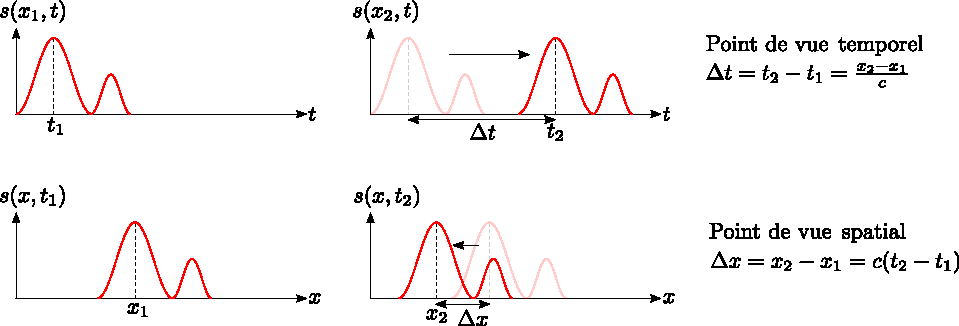
\includegraphics[width=\textwidth]{Figures/OPP.pdf}
  \caption{Représentation d'une onde progressive. Le signal mesuré au point $x_1$ à l'instant $t_1$ est identique à celui mesuré au point $x_2$ à l'instant $t_2$, les décalages en temps et en espace étant reliés par la vitesse de l'onde $c$. La figure du haut représente une onde progressive vers les $x$ croissants, en point de vue temporel (on place deux capteurs, en $x_1$ et $x_2$, et on enregistre l'onde au cours du temps), alors que la figure du bas représente une onde régressive (ou progressive selon les $x$ décroissants) en point de vue spatial (on prend deux photos de l'onde, en $t_1$ et $t_2$, et on enregistre l'évolution de l'onde dans tout l'espace).}
  \end{figure}
  

\begin{exemple}{Solution en ondes planes progressives}
  On rappelle la formule de la dérivée en chaîne d’une fonction composée $f(u(x))$,
  $$
  % \eqbox{
    \frac{\d f}{\d x} = \frac{\d f}{\d u}\frac{\d u}{\d x} = f'(u(x))u'(x).  
    % }
  $$
  On considère une OPP de la forme $s(x,t) = f(x-ct)$.
  \begin{quest}
    \item	 Calculer les dérivées partielles $\dr{s}{x}$ et $\ddr{s}{x}$.
    \item Calculer les dérivées partielles $\dr{s}{t}$ et $\ddr{s}{t}$.
    \item Montrer que $s(x,t)$ est solution de l’équation de d’Alembert.
  \end{quest}

  \examplesol{
    \begin{quest}
      \item	Par la règle de dérivation en chaîne,
      \begin{equation*}
        \dr{s}{x}(x,t) = f’(x-ct) \text{ et } \ddr{s}{x}(x,t) = {f}^{\prime\prime}(x-ct).
      \end{equation*}
      \item Par la règle de dérivation en chaîne,
      \begin{equation*}
        \dr{s}{t}(x,t) = -c f’(x-ct) \text{ et } \ddr{s}{t}(x,t) = c^2 {f}^{\prime\prime}(x-ct).
      \end{equation*}
      \item
      On a bien que
      \begin{equation*}
        \dr{s}{x}(x,t) - \frac{1}{c^2} \ddr{s}{t}(x,t) =  {f}^{\prime\prime}(x-ct) - f^{\prime\prime}(x-ct) = 0.
      \end{equation*}
    \end{quest}
  }
\end{exemple}
% Une première famille de solutions de l'équation d'onde sont les ondes planes progressives de la forme
% \begin{equation}
% \label{eq:OPP}
% s(x,t)=f_1(x-ct)+g_1(x+ct)=f_2(t-\frac{x}{c})+g_2(t+\frac{x}{c}),
% \end{equation}
% où les fonctions $f$ et $g$ sont quelconques (mais en tant que fonctions physiques, elles sont au moins dérivables deux fois par rapport à l'espace et au temps). La première écriture avec $(f_1,g_1)$ privilégie une interprétation spatiale, tandis que la deuxième $(f_2,g_2)$ se prête davantage à une interprétation temporelle.
% Il est facile de vérifier que l'expression \eqref{eq:OPP} est solution de l'équation de d'Alembert.

Nous admettrons de plus que \important{toutes} les solutions de l'équation de d'Alembert peuvent se mettre sous la forme d’une somme d’ondes planes progressives se propageant en sens opposées. On dit que les ondes planes progressives forment une base de solutions.

\begin{prop}[Base des solutions en OPP]\label{prop:}
  Toute solution de l’équation de d’Alembert se met sous la forme d'une combinaison linéaire d'OPP
  $$
  s(x,t)=f(x-ct)+g(x+ct).
  $$
\end{prop}


\subsection{Ondes planes progressives harmoniques (OPPH)}
\parag{Définition} Pour l'instant nous n'avons pas spécifié de fonction $f$ ou $g$ particulière. Un cas important d'OPP est celle telle que la fonction $f$ ou $g$ sinusoïdale.
\begin{definition}[OPPH]
  Une \imp{onde plane progressive harmonique} est une OPP (selon les $x$ croissants ici)  de la forme
  \begin{equation*}
   s(x,t)=s_m\cos(\omega t-kx+\varphi),
 \end{equation*}
 de pulsation $\omega$ (en $\SI{}{rad.s^{-1}}$), vecteur d'onde $k$ (en $\SI{}{m^{-1}}$), amplitude $s_m$, et phase à l’origine $\varphi$.
\end{definition}


 Cette expression est-elle toujours solution de l'équation de d'Alembert ? A priori non, car nous avons vu qu'elle doit se mettre sous la forme d'une fonction de $x-ct$. Or la phase $\omega t-kx=-k(x-\frac{\omega}{k}t)$ est de la forme $-k(x-ct)$ à condition que
% \begin{equation}
\eqbox[]{
  \omega = k c.
  }
%  \end{equation}
 L'OPPH soit solution de l'équation de d'Alembert si elle vérifie cette relation algébrique entre $k$ et $\omega$, appelée \important{relation de dispersion}. Ici, la relation de dispersion est linéaire puisque $\omega$ est proportionnel à $k$.

 \begin{theorem}[Relation de dispersion]\label{form:}
  On appelle \imp{relation de dispersion} une relation algébrique entre la pulsation $\omega$ et le vecteur d'onde $k$.
Une OPPH est solution de l’équation de d’Alembert si elle vérifie la relation de dispersion
$$
  \omega = k c.
$$
 \end{theorem}

\begin{remarque}
 Il s'agit d'une propriété générale de l'équation de d'Alembert, nous verrons dans la suite que la conséquence d'une relation de dispersion linéaire est que la vitesse de propagation des ondes est identique quelle que soit leur fréquence. On parle alors de propagation sans dispersion. Mais cela ne sera pas toujours le cas avec d'autres équations d'onde (voir les chapitres suivants)!
 \end{remarque}

\parag{Propriétés}
Une OPPH est une fonction doublement périodique.
\begin{liste}
  \item La période temporelle est donnée par la période $T = \frac{2\pi}{\omega}$. 
  \item La période spatiale est donnée par la longueur d'onde $\lambda = \frac{2\pi}{k}$.
\end{liste}
% La grandeur $k=\frac{2\pi}{\lambda}$ désigne , $\lambda$ la longueur d'onde (spatiale) de l'onde, $T=\frac{1}{f}=\frac{2\pi}{\omega}$ la période temporelle de l'onde, $f$ sa fréquence et $\omega$ sa pulsation. On dit que l'onde plane progressive possède une \important{double périodicité}: spatiale ($k=\frac{2\pi}{\lambda}$) et temporelle ($\omega=\frac{2\pi}{T}$).
Les OPPH solutions de l’équation de d’Alembert vérifient donc $\lambda=cT$, ce qui provient de la relation de dispersion $\omega=ck$. Ce lien est donc une conséquence de l'équation de d'Alembert.

% \parag{Détermination d’une relation de dispersion}
% Considérons une équation d'onde linéaire. Nous pouvons alors utiliser la notion complexe et écrire \emph{dans le cas d'une OPPH} se propageant selon les $x$ croissants, le signal $s(x,t)$ comme la partie réelle de
% \begin{equation}
%   \underline{s}=s_0\e^{i\varphi}\e^{i(\omega t-kx)}.
% \end{equation}
% Avec cette convention, nous avons l’équivalence
% \begin{equation}
%    \frac{\partial}{\partial t}\Leftrightarrow \times \,i\omega \text{ et } \frac{\partial}{\partial x}\Leftrightarrow \times\, -ik.
% \end{equation}
%  En remplaçant dans l'équation de d'Alembert on obtient que $\underline{s}$ est solution si et seulement si $k^2=\frac{\omega^2}{c^2}$, et on prendra $k=+\frac{\omega}{c}$ pour que l'onde se propage selon les $x$ croissants.
% \begin{remarque}
% L'équation de d'Alembert étant particulièrement simple, on peut travailler directement avec l'expression réelle $s_0\cos(\omega t-kx+\varphi)$ et remplacer dans l'équation de d'Alembert. Mais le réflexe de passer en complexes fonctionne toujours, et s'avère quasiment indispensable dans les cas plus compliqués.
% \end{remarque}


\subsection{Ondes planes stationnaires (OPS)}

\parag{Définition} Stationnaire signifie de façon générale « indépendant » du temps. Dans le cas d'une onde, ce n'est pas la fonction $s(x,t)$ elle-même qui est indépendante du temps (sinon il n'y a pas d'onde!), mais la position des maxima (ventres) et minima (nœuds) de l'onde.

\begin{definition}[OPS]\label{def:}
  Une \imp{onde plane stationnaire} est une onde dont les dépendances spatiale et temporelle sont découplées :
  \begin{equation*}
  \label{eq:OS}
  s(x,t)=f(x)g(t).
  \end{equation*}
\end{definition}



% \begin{remarque}
% Ne \important{surtout pas} croire qu'une onde stationnaire ne dépend pas du temps ! C'est une onde, donc elle dépend nécessairement de l'espace et du temps, c'est d'ailleurs visible dans l'expression \eqref{eq:OS}. Une onde stationnaire est seulement une onde pour lesquelles les variations spatiales et temporelles sont \important{découplées}.
% \end{remarque}
\noindent
Montrons à quelle condition sur $f$ et $g$ une onde stationnaire est solution de l'équation de d'Alembert. 
% En substituant on obtient

\begin{demo}
\begin{equation}
  g(t)f^{\prime \prime}(x)-\frac{1}{c^2}f(x)g^{\prime \prime}(t)=0\quad\Leftrightarrow\quad \frac{f^{\prime \prime}(x)}{f(x)}=\frac{1}{c^2 }\frac{g^{\prime \prime}(t)}{g(t)}=\cte.
\end{equation}
% puisque qu'une fonction du temps ne peut être égale à une fonction de l'espace que si ces fonctions sont égales à une constante (indépendante du temps et de l'espace).
Quel peut-être le signe de cette constante ? Si elle était positive, $g(t)$ serait exponentielle. Si l'exponentielle diverge, l'onde n'est pas physique ; si elle  s'atténue, l'onde n'est pas stationnaire. On rejette donc ce cas et on pose $\cte = -k^2 < 0$.  Par analyse dimensionnelle, $k$ est homogène à un vecteur d'onde. L'équation
\begin{equation}
  f^{\prime \prime}(x) +k^2 f(x) = 0
\end{equation}
est celle d'un oscillateur harmonique, de solution $f(x)=s_m\cos(kx+\vphi)$. En posant $\omega =ck$ on en déduit de même $g(t)=\cos(\omega t+\psi)$.
\end{demo}
% La solution générale se met donc sous la forme
% \begin{equation}
% \begin{split}
% s(x,t)&=s_m\cos(kx+\psi)\cos(\omega t+\varphi).
% \end{split}
% \end{equation}
Comme $f$ et $g$ sont des fonctions sinusoïdales, l'onde stationnaire est harmonique.
\begin{prop}[Solution stationnaire de l'équation de d'Alembert]\label{prop:}
  Une OPS solution de l'équation de d'Alembert est \imp{harmonique} et vérifie $\omega =k c $, soit
  \begin{equation*}
  s(x,t)=s_m\cos(kx+\psi)\cos(\omega t+\varphi).
\end{equation*}
\end{prop}

\parag{Propriétés}

L'amplitude$f(x)=s_m\cos(kx+\psi)$ dépend donc de l'espace : tous les points vibrent en phase, mais à une amplitude différente. On distingue deux types de points d'amplitudes particulières.

\begin{liste}
  \item Un \imp{ventre} est une position $x_v$ d'amplitude extrémale (maximale ou minimale). Ainsi $f(x_v) = \pm s_m$ et donc $kx_{\rm{v}}+\vphi=p\pi$ avec $p\in\mathbb{Z}$, soit en supposant $\vphi=0$ pour simplifier,
% \begin{equation}
  \eqbox[]{
    x_{\rm{v}}=\frac{\lambda}{2}p,
  }
% \end{equation}
avec $k=\frac{2\pi}{\lambda}$. Les ventres sont donc séparées d'une demi-longueur d'onde $\lambda/2$.
\item Un \important{nœud}  est une position $x_n$ où l'amplitude est nulle. Ainsi $f(x_n)=0$ et donc $kx_{\rm{n}}=(2p+1)\frac{\pi}{2}$ avec $p\in\mathbb{Z}$, d'où
% \begin{equation}
  \eqbox[]{
    x_{\rm{n}}=\frac{\lambda}{2}\left(p+\frac{1}{2}\right).
  }
% \end{equation}
Les nœuds sont donc aussi séparés d'une demi-longueur d'onde $\lambda/2$. Les ventres et les nœuds sont séparés entre eux d'une quart de longueur d'onde $\lambda/4$.
\end{liste}


% \begin{figure}[h!]
% \centering
% 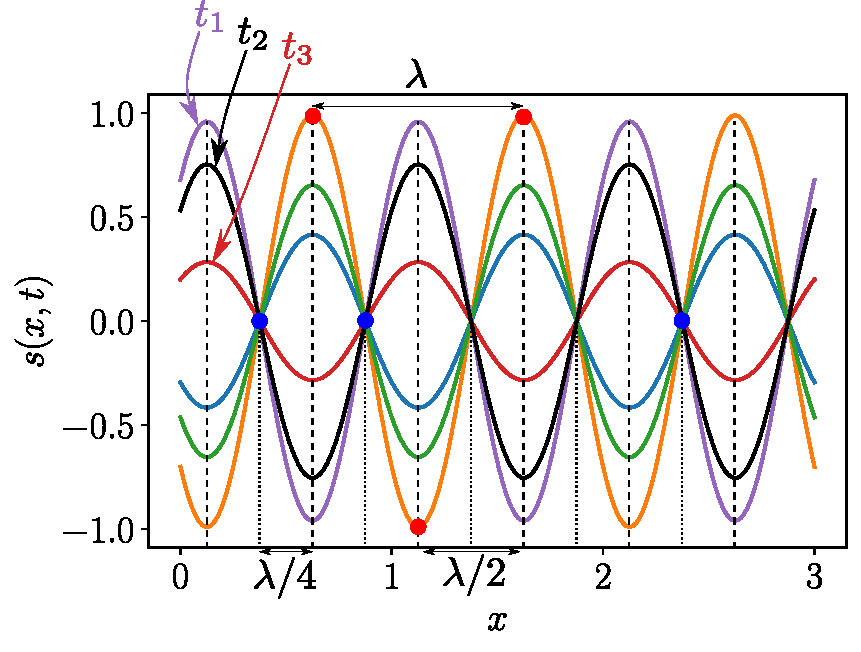
\includegraphics[width=0.6\textwidth]{Figures/onde_stationnaire.pdf}
% \caption{Représentation d'une onde stationnaire de la forme $s(x,t)=\cos(kx+\psi)\cos(\omega t+\varphi)$ à différents instants.}% avec $\psi=-\frac{\pi}{4}$, $\varphi=0$, $\lambda=\SI{1}{m}$ et $T=\SI{2\pi}{s}$. Ainsi les instants $t_i$ représentés sont tels que $t_i=(i+1)$ (en seconde).}
% \end{figure}

\begin{figure}[H]
  \centering
  
\includegraphics{standing_wave.pdf}
  \caption{Représentation d'une OPS harmonique. Les courbes pleines représente l'amplitude de l'onde $f(x) = s_m\cos(k x)$ et son opposé. Les courbes pointillées représentent l'OPS $s(x,t)=f(x) \cos(\omega t)$ à différents instants. Les nœuds sont séparés entre eux d'une demi-longueur d'onde $\lambda/2$, de même que les ventres.}
  \label{}
\end{figure}


\section{Modes propres d'une corde vibrante fixée}

\subsection{Régime libre}
\parag{Position du problème}
Pour résoudre complètement l’équation de d’Alembert, nous devons lui adjoindre des \imp{conditions aux limites}. Dans un régime \imp{libre}, nous fixons la corde vibrante  de longueur $L$ fixée à ses deux extrémités, de sorte que
% \begin{equation}
  \eqbox[]{
    \forall t, y(x=0,t)=0 \text{  et  } y(x=L,t)=0.
  }
% \end{equation}
On dit dans ce cas que l'onde est \imp{confinée}.
On suppose qu'on écarte la corde de sa position d'équilibre, par exemple en donnant
 une percussion à la corde, puis on étudie l’évolution de la corde dans le temps.

 \begin{definition}[Régime libre]\label{def:}
  Un système éloigné de l’équilibre qui évolue sans apport d’énergie obéit au \imp{régime libre}.
 \end{definition}
 L'évolution libre est alors régie par l'équation d'onde et les \imp{conditions initiales}. Comme l'équation de d'Alembert est linéaire d'ordre $2$, une condition initiale doit préciser 
 \begin{liste}
  \item
  l'amplitude initiale $y(x,t=0)$ ;
  \item la vitesse initiale $\dr{y}{t}(x,t=0)$.
 \end{liste}

\begin{exemple}{Corde d'instrument de musique}
Dans un instrument à cordes pincées, comme le clavecin, la corde est déformée puis lâchée sans vitesse initiale. Dans un instrument à cordes frappées, comme le piano, le musicien communique une vitesse initiale à une corde non déformée. Que dire des conditions initiales dans ces deux cas ?

\examplesol{
  \begin{liste}
    \item
    la corde est déformée ($y(x,t=0) \neq 0$) puis lâchée sans vitesse initiale ($\dr{y}{t}(x,t=0)=0$).
    \item le musicien communique une vitesse initiale ($\dr{y}{t}(x,t=0) \neq 0$) à une corde non déformée ($y(x,t=0) = 0$).
  \end{liste}
}
\end{exemple}
%  de sort $y(x,0)\neq 0$ et $\frac{\partial y}{\partial t}(x,0)\neq 0$. On
%
% Dans la suite nous allons rechercher les conditions que doivent satisfaire le module du nombre d'onde $k$ (ou de façon équivalente $\omega$ d'après la relation de dispersion) pour que des ondes apparaissent. Nous allons montrer que de façon très générale, les contraintes imposées à l'onde par les conditions aux limites vont sélectionner certaines fréquences particulières. Le nombre de fréquences autorisées est discret: on parle de quantification par les conditions aux limites. Il s'agit d'une propriété très générale des ondes et des oscillateurs en général, que nous retrouverons dans le cadre de la mécanique quantique.

\parag{Modes propres et quantification}

Comme les extrémités de la corde sont fixées en $x=0$ et $x=L$, on s'attend à ce que l'onde soit stationnaire et que les extrémités correspondent à des nœuds de l'onde.
On cherche donc une solution sous la forme
\begin{equation}
  y(x,t)=A\cos(kx+\psi)\cos(\omega t+\vphi),
\end{equation}
où $\omega = k c$ pour satisfaire à l'équation de D'Alembert. On montre alors que $\omega$ et $k$ sont quantifiés.

\begin{demo}
Pour satisfaire les \udl{conditions aux limites fixes}, il faut
\begin{equation}
  \left\{\begin{array}{cc}
y(0,t) & = 0\\
\dr{y}{t}(0,t) & = 0
\end{array}\right. \forall t
\Rightarrow
\left\{\begin{array}{cc}
A \cos(\psi)\cos(\omega t + \vphi) & = 0\\
A \omega \cos(kL + \psi)\sin(\omega t + \vphi) & = 0
\end{array}\right. \forall t.
\end{equation}
On a bien sûr $A \neq 0$ pour obtenir une solution non triviale. La seule possibilité est donc que
\begin{equation}
  \left\{
    \begin{array}{cc}
    \cos \psi & = 0 \\ 
    \cos(k L + \psi) & = 0\\ 
    \end{array}
  \right. 
  \Rar
  \left\{
    \begin{array}{cc}
    \psi=(2p+1)\frac{\pi}{2},  p\in\mathbb{Z} \\ 
    \cos(kL+2(p+1)\frac{\pi}{2}) =\sin(kL)  = 0\\ 
    \end{array}
  \right. 
\end{equation}
La dernière condition impose $kL=n\pi$ avec $n\in\mathbb{N}^{\star}$, soit 
\eqbox[]{
k = \frac{n\pi}{L}.
}
La pulsation est aussi quantifiée d’après la relation de dispersion, 
\eqbox[]{
\omega =\frac{n \pi c}{L}.
}
Les modules du vecteur d'onde ne peuvent prendre que certaines valeurs qui dépendent d'un nombre entier $n\in\mathbb{N}^{\star}$
: on dit qu'ils sont \important{quantifiés}. 
\end{demo}


\begin{prop}[Modes propres]\label{prop:}
  Les solutions de l'équation de d'Alembert avec conditions aux limites \imp{fixes}  sont les \imp{modes propres}.
  
  Les modes propres sont \imp{quantifiés} par un entier  $n \in \N^*$ tel que
  \begin{equation*}
    k_{n}=n\frac{\pi}{L} \quad \text{et} \quad \omega_{n}=n\frac{\pi c}{L},
  \end{equation*}

\end{prop}
En conséquence, la longueur d'onde est quantifiée et vérifie $L = n \frac{\lambda_n}{2}$. La déformation de la corde du mode $n$ est donc constitué de $n$ faisceaux.
% $\lambda_{n}=\frac{2L}{n}.$
%
% La quantification des vecteurs d'onde conduit également d'après la relation de dispersion à une quantification des fréquences de l'onde
% \begin{equation}
%   k_{n}=n\frac{\pi}{L} \quad \Leftrightarrow\quad \omega_{n}=n\frac{\pi c}{L} \quad \Leftrightarrow \quad \lambda_{n}=\frac{2L}{n}.
%   \end{equation}
% Ces conditions de quantification définissent les conditions d'existence d'une onde stationnaire dans une cavité spatialement limitée (ici entre les deux points d'attache de la corde).
Les modes propres $y_{n}(x,t)$ ont donc pour expression
\begin{equation}
 y_{n}(x,t)=A_{n}\sin\left(n\frac{\pi}{L}x\right)\cos\left(n\frac{\pi c}{L}t + \vphi \right).
 \end{equation}
 \begin{liste}
  \item
  Le mode propre $n=1$, de pulsation $\omega_1 = \frac{\pi c}{L}$, est appelé mode \imp{fondamental}. 
  \item Les modes propres pour $n>1$ sont appelés \imp{harmoniques}.
\end{liste}
  % où $n\in\mathbb{N}^{\star}$ sont appelées les \important{modes propres}, et les pulsations $\omega_{n}=n\frac{\pi c}{L}$ sont appelées les pulsations propres. La plus petite pulsation ($n=1$) est appelée le fondamental, et les $n>1$ les harmoniques.

 \begin{figure}[h!]
 \centering
 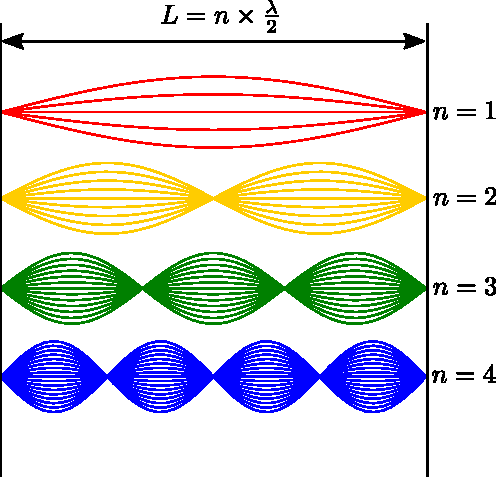
\includegraphics[width=0.45\textwidth]{Figures/modes_OS.pdf}
 \caption{Représentation des premiers modes d'une onde stationnaire dans une cavité de longueur $L$. La couleur illustre la variation en longueur d'onde par analogie avec la variation observée dans le domaine de la lumière visible ($\lambda_{n}=\frac{2L}{n}$, si $n$ augmente, $\lambda$ diminue et tire de plus en plus vers le violet).}
 \end{figure}

%  \begin{remarque}
%  On peut illustrer un grand nombre de phénomènes sur l'exemple de la guitare. Les fréquences autorisées dépendent de la longueur des cordes par $f_{n}=\frac{nc}{2L}$ où $L$ est la longueur de la corde et $c$ est la vitesse des ondes acoustiques dans la corde, qui vaut $\sqrt{\frac{T}{\mu}}$ avec $T$ sa tension et $\mu$ sa masse linéique. Pour accorder une guitare, on tourne une molette qui a pour effet d'enrouler la corde autour d'un petit cylindre, et donc de la tendre ou de la détendre selon le sens de l'enroulement. Si on tend la corde ($T$ augmente), la vitesse de propagation des ondes $c$ augmente et donc la fréquence augmente: on a un son plus aigu. C'est d'ailleurs aussi le principe de fonctionnement d'un vibrato sur les guitares électriques: qui tend ou détend les cordes et fait donc osciller la fréquence autour d'une valeur moyenne. Pour la guitare, la longueur à vide des cordes est fixée (autour de \SI{65}{cm}) donc le dernier paramètre sur lequel on peut jouer pour changer la fréquence est la masse linéique $\mu$. Plus la masse linéique est élevée, plus la fréquence est faible et donc plus le son est grave: c'est pourquoi les cordes n'ont pas toutes la même épaisseur.
%  Enfin, lorsqu'on pince une corde à un endroit donné, on fait varier la longueur $L$ de la corde et donc la fréquence jouée est modifiée. (En réalité, c'est un tout petit peu plus complexe: d'une part les harmoniques suivantes sont en principe aussi présentes, mais on peut montrer que leur amplitude décroît avec $n$ de sorte qu'elles sont moins audibles que la fréquence fondamentale; d'autre part la composition en harmonique exacte du son émis dépend aussi de l'endroit où on attaque (pince ou frappe) la corde, car on annule toutes les harmoniques qui ont un nœud au point frappé.)

%  Sur les guitares, il existe des petites tiges métalliques (les frètes) qui permettent d'assurer que la longueur soit fixée à une valeur très précise tant que le doigt qui appuie se situe entre deux frètes. Ceci n'est pas le cas de tous les instruments à corde, comme par exemple le violon. C'est aussi pourquoi jouer une fréquence précise est beaucoup plus difficile au violon qu'à la guitare (mais c'est aussi pourquoi le spectre en fréquence d'un violon est infiniment plus riche que celui d'une guitare, puisqu'en principe $L$ peut varier continûment).
%  \end{remarque}

 \subsection{Régime forcé}
On impose maintenant des conditions aux limites mixtes, avec une extrémité fixe en $x=L$, l’extrémité $x=0$ étant excité par un pot vibrant. Les conditions aux limites pour ce \imp{régime forcé} s’écrivent donc 
% \begin{equation}
\eqbox[]{
  \forall t, y(0,t)=a\cos(\omega t) \text{ et } y(L,t)=0,
  }
% \end{equation}

  \begin{experience}{La corde de Melde}\label{exp:}
    
    
    % {
    

    On considère une corde de longueur $L=\SI{89}{cm}$ où une extrémité est fixée par une masse $m=\SI{50}{g}$, tandis que l'autre extrémité est attachée à un pot vibrant de sorte que son amplitude varie de façon forcée comme $y(x=0,t)=a\cos(\omega t)$. La tension du fil est imposée par le poids de la masselotte. 
    Nous allons montrer qu'il apparaît un phénomène intéressant si l'excitation se fait sur un mode propre de la corde. Une corde vibrante excitée de cette façon est appelée \imp{corde de Melde}.
    \begin{wrapfigure}{r}{0.4\textwidth}
    
\includegraphics[width=0.4\textwidth]{path38425-6.pdf}
    \end{wrapfigure}
    % }

    
    %  \begin{figure}[h!]
      %  \centering
      \begin{quest}
        \item	Calculer la tension $T$ puis la célérité $c=\sqrt{T/\mu}$.
        \item Donner l’expression de la fréquence propre $f_n$. Calculer la fréquence fondamentale $f_1$. 
        \item Comment observer expérimentalement les modes propres de la corde ? Comparer la valeur mesurée de $f_1$ à la valeur attendue.
      \end{quest}
    %   \begin{fig}[label]
    %   \centering
    %   %\capt{}
    %   
\includegraphics[width=0.7\textwidth]{pot_vibrant.pdf}
    %   % \capt{Étude expérimentale des oscillations forcées d'une corde.}
    % \end{fig}
    \examplesol{
      \begin{quest}
        \item	On trouve
      \end{quest}
    }
   %  \end{figure}
  \end{experience}
  
\begin{prop}[Résonance en régime forcée]\label{prop:}
  L'amplitude de la  déformation corde vibrante en régime forcée diverge lorsque la corde est excitée à une fréquence propre $\omega_n$. On dit qu'il y a \imp{résonance}, car le transfert d’énergie est maximal.
\end{prop}

\begin{demo}
  \textsl{}
  \begin{enumerate}
    \item \udl{Forme de la solution}.
 Puisqu'il existe un nœud en $x=L$, cherchons la solution sous la forme d'une onde stationnaire
\begin{equation}
  y(x,t)=A\cos(kx+\psi)\cos(\omega t+\vphi).
\end{equation}
  \item \udl{Condition en $x=0$}. On a $A\cos(\omega t+\vphi)\cos(\psi)=a\cos(\omega t)$ ce qui impose que $\vphi=0$ et $a=A\cos(\psi)$, soit 
  \eqbox{
  A = \frac{a}{\cos \psi}.
  }
  \item \udl{Condition en $x=L$}. On a  $\forall t$, $A\cos(\omega t)\cos(kL+\psi)=0$ et donc 
  \eqbox{
    \psi=-kL+(2p+1)\frac{\pi}{2}, p\in\mathbb{Z}^{\star}.
    }
    \item \udl{Solution exacte}.
    La vibration de la corde s’écrit donc
    \begin{equation}
      \begin{split}
        y(x,t)&=\frac{a}{\cos(\psi)}
        \cos(\omega t){\cos(k(x-L)+(2p+1)\frac{\pi}{2})}
      \end{split}
    \end{equation}
    Or $\cos(\theta-(2p+1)\frac{\pi}{2})=(-1)^{p}\sin(\theta)$  pour tout $\theta$, de sorte que
    % \begin{equation}
    \eqbox[]{
      y(x,t)    =\frac{a}{\sin(kL)}\sin(k(L-x))\cos(\omega t).
      }
    \end{enumerate}
      % \end{equation}
      On remarque que l'amplitude de l'onde sur la corde diverge lorsque $\sin(kL)=0$ c'est-à-dire pour $kL=n\pi$ avec $n\in\mathbb{N}^{\star}$, ce qui correspond aux modes propres, de vecteurs d'ondes $k_n = n \frac{\pi}{L}$. Cela est possible si la pulsation vaut $\omega=\omega_n=n\frac{\pi c}{L}$. Il y a donc \imp{résonance} lorsque la fréquence d’excitation égale la fréquence propre.
\end{demo}

% test
%    Il y a un phénomène de \important{résonance} lorsque la pulsation d'excitation $\omega$ du vibreur coïncide avec celle d'un mode propre $\omega_n=n\frac{\pi c}{L}$.
  \begin{remarque}
  En pratique, la divergence est limitée par la dissipation énergétique et les effets non linéaires, que nous n'avons pas pris en compte dans l'équation d'onde de d'Alembert.
  \end{remarque}

\end{document}
